\documentclass[11pt]{article}

\usepackage[margin=0.9in]{geometry}
\usepackage{amsmath,amssymb,amsthm,mathtools}
\usepackage{graphicx}
\usepackage{microtype}
\usepackage{xcolor}
\usepackage{enumitem}
\usepackage[hidelinks]{hyperref}

\newtheorem{theorem}{Theorem}
\newtheorem{lemma}{Lemma}
\newcommand{\C}{\mathbb C}
\newcommand{\R}{\mathbb R}
\newcommand{\Tr}{\operatorname{Tr}}
\newcommand{\diag}{\operatorname{diag}}
\newcommand{\ran}{\operatorname{ran}}
\newcommand{\cbF}{\mathrm{cbF}}
\newcommand{\F}{\mathrm{F}}

\title{Haagerup's Constructive Vector Need Not Be cbF-Optimal\\
\large An explicit rank-two projection counterexample to a question in arXiv:2312.09029}
\author{Automated mathematics run \texttt{fa\_banach\_001}, lane 14}
\date{21 July 2026}

\begin{document}
\maketitle

\begin{center}
\fcolorbox{black}{gray!8}{\parbox{0.88\textwidth}{
\textbf{Status.} Candidate full counterexample, likely valid, pending human
review.  The proof is exact; numerical optimization is used only as an
independent sanity check.
}}
\end{center}

\section{Source question}

The source is Erik Christensen, \emph{Some points of view on Grothendieck's
inequalities}, arXiv:2312.09029 \cite{Christensen2024}.  The introduction asks
whether Haagerup's method actually produces the optimal cbF-factorization (or
the corresponding operator factorization) of a complex matrix.  In Section 3,
after proving optimality for matrices with nonnegative entries, the paper says
that in the general case Haagerup's vector might remain optimal, but the author
expects otherwise and has no definite result.  The passage begins at the foot
of p.~11 and continues on p.~12 of the arXiv PDF:

\begin{figure}[htbp]
  \centering
  
\includegraphics[width=\textwidth]{figures/open_problem_crop_page11.png}
  \vspace{0.35em}
  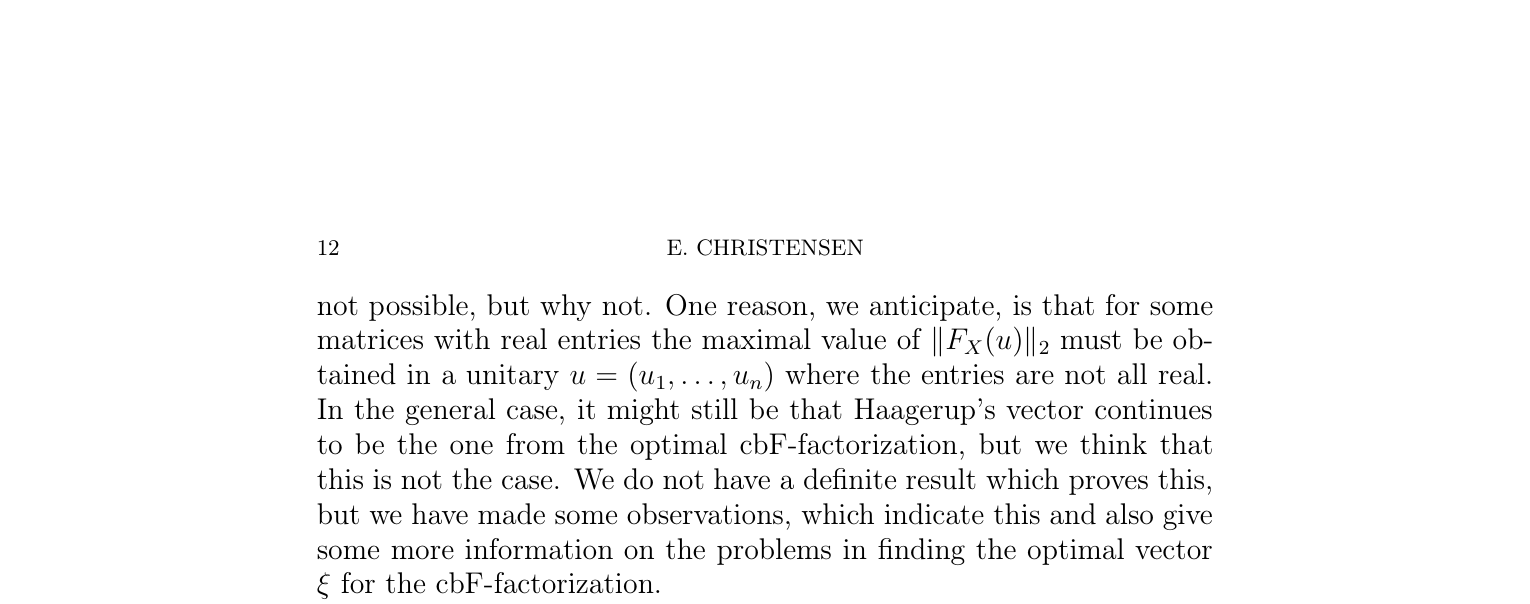
\includegraphics[width=\textwidth]{figures/open_problem_crop_page12.png}
  \caption{Full-width crops from pp.~11--12 of the source PDF.}
  \label{fig:source-question}
\end{figure}

The relevant general-case sentence is:
\begin{quote}
``In the general case, it might still be that Haagerup's vector continues to
be the one from the optimal cbF-factorization, but we think that this is not
the case. We do not have a definite result which proves this.''
\end{quote}

We give the requested definite negative result.

\section{Definitions and an equivalent diagonal optimization}

For $z\in\C^n$, write $\Delta(z)$ for the diagonal matrix with diagonal $z$.
For a complex $m\times n$ matrix $X$, the source's factorization norm can be
written as
\begin{equation}
 \|X\|_{\cbF}
 =\min_{\substack{\xi\in\R_+^n\\ \|\xi\|_2=1}}
   \bigl\|X\Delta(\xi)^{-1}\bigr\|_{\mathrm{op}},
 \label{eq:cbf-factor}
\end{equation}
with the usual support convention if a coordinate of $\xi$ vanishes.  In our
example every feasible diagonal below is strictly positive, so no support
subtlety occurs.

The ordinary $F$-norm is
\[
 \|X\|_{\F}=\max_{|u_j|=1}\|Xu\|_2.
\]
For a maximizing unimodular vector $u$, Haagerup's construction assigns the
probability vector
\begin{equation}
 \lambda_j=\frac{\overline{u_j}(X^*Xu)_j}{\|X\|_{\F}^2},
 \qquad \xi_{H,j}=\sqrt{\lambda_j}.
 \label{eq:haagerup}
\end{equation}
The maximizing property makes the $\lambda_j$ real and nonnegative, and their
sum is one; this is precisely the state construction in Section 3 of the
source \cite{Christensen2024}.

\begin{lemma}[Diagonal SDP form]
For $P=X^*X$,
\begin{equation}
 \|X\|_{\cbF}^2
 =\min\{\Tr D: D\text{ is diagonal and }D\succeq P\}.
 \label{eq:sdp}
\end{equation}
If $\xi$ is optimal in \eqref{eq:cbf-factor} and
$t=\|X\|_{\cbF}^2$, then $D=t\Delta(\xi)^2$ is optimal in
\eqref{eq:sdp}.  Conversely, an optimal $D$ of trace $t$ gives the optimal
vector $\xi_j=\sqrt{D_{jj}/t}$.
\end{lemma}

\begin{proof}
For a positive unit vector $\xi$, put
\[
 t(\xi)=\|X\Delta(\xi)^{-1}\|_{\mathrm{op}}^2
 =\|\Delta(\xi)^{-1}P\Delta(\xi)^{-1}\|_{\mathrm{op}}.
\]
The inequality
$\Delta(\xi)^{-1}P\Delta(\xi)^{-1}\preceq t(\xi)I$
is equivalent to
$P\preceq t(\xi)\Delta(\xi)^2$.  Thus
$D=t(\xi)\Delta(\xi)^2$ is feasible and
$\Tr D=t(\xi)$.  Conversely, if diagonal $D\succeq P$ has trace $t$, set
$\xi_j=\sqrt{D_{jj}/t}$.  Then $\|\xi\|_2=1$ and
$P\preceq t\Delta(\xi)^2$, so $t(\xi)\le t$.  Taking minima in both
directions proves \eqref{eq:sdp} and the optimizer correspondence.
\end{proof}

\section{Proof intuition}

We design a two-dimensional subspace $L\subset\C^4$ with two competing
properties.  First, $L$ has a positive frame operator $Q$ whose four diagonal
entries are all one.  This gives an exact dual witness forcing the unique
optimal diagonal in \eqref{eq:sdp} for the projection onto $L$ to be $I_4$;
hence the unique optimal factorization vector is uniform.  Second, $L$ has no
unimodular vector.  If Haagerup's weights were uniform, the maximizing
unimodular vector in \eqref{eq:haagerup} would have to be a nonzero eigenvector
of the projection with eigenvalue in $(0,1]$, forcing it into $L$.  The two
properties are incompatible, so Haagerup's vector cannot be optimal.

\section{The counterexample}

\begin{theorem}
Let
\begin{equation}
 A=\begin{pmatrix}
 1&0\\
 0&1\\
 2^{-1/2}&2^{-1/2}\\
 2^{-1/2}&i2^{-1/2}
 \end{pmatrix},
 \qquad
 P=A(A^*A)^{-1}A^*.
 \label{eq:A-P}
\end{equation}
Then $P$ is a $4\times4$ orthogonal projection of rank two.  For $X=P$,
the cbF-optimal positive unit vector is uniquely
\[
 \xi_0=\tfrac12(1,1,1,1),
 \qquad \|P\|_{\cbF}^2=4.
\]
For every maximizing unimodular vector $u$ used in Haagerup's construction,
the vector $\xi_H$ from \eqref{eq:haagerup} differs from $\xi_0$.
Consequently Haagerup's cbF-factorization, and hence its corresponding
operator factorization, is strictly nonoptimal for this explicit matrix.
\end{theorem}

\begin{proof}
The range of $A$ is
\begin{equation}
 L=\left\{\left(a,b,\frac{a+b}{\sqrt2},
                 \frac{a+ib}{\sqrt2}\right):a,b\in\C\right\}.
 \label{eq:L}
\end{equation}
The two columns of $A$ are independent, so \eqref{eq:A-P} is the orthogonal
projection onto $L$.

We first show that $L$ contains no unimodular vector.  If a vector in
\eqref{eq:L} had all four coordinates of modulus one, then $|a|=|b|=1$.
The third coordinate would give
\[
 |a+b|^2=2 \quad\Longrightarrow\quad \Re(a\overline b)=0,
\]
while the fourth would give
\[
 |a+ib|^2=2 \quad\Longrightarrow\quad \Im(a\overline b)=0.
\]
This is impossible because $|a\overline b|=1$.

Now put $Q=AA^*$.  Each row of $A$ has Euclidean norm one, so
\begin{equation}
 Q\succeq0,\qquad \diag(Q)=(1,1,1,1),\qquad \ran Q=L.
 \label{eq:Qfacts}
\end{equation}
Since $P$ is the projection onto $L$, we have $PQ=Q$, and therefore
\begin{equation}
 \Tr(PQ)=\Tr Q=4.
 \label{eq:PQtrace}
\end{equation}
The diagonal $D=I_4$ is feasible in \eqref{eq:sdp}, because $P\preceq I_4$.
For any other feasible diagonal $D\succeq P$, positivity and
\eqref{eq:Qfacts}--\eqref{eq:PQtrace} give
\[
 0\le\Tr((D-P)Q)
   =\sum_{j=1}^4D_{jj}Q_{jj}-\Tr(PQ)
   =\Tr D-4.
\]
Thus the minimum in \eqref{eq:sdp} is $4$.

It is also unique.  If equality holds, the positive matrices $D-P$ and $Q$
satisfy $\Tr((D-P)Q)=0$.  Hence
$Q^{1/2}(D-P)Q^{1/2}=0$, which implies that $D-P$ annihilates
$\ran Q=L$.  On $L$ the projection $P$ is the identity, so $Dv=v$ for every
$v\in L$.  Every coordinate is nonzero on some vector of $L$; since $D$ is
diagonal, this forces $D_{jj}=1$ for all $j$.  Therefore $D=I_4$ is the
unique optimizer.  By the diagonal SDP lemma, the unique optimal
factorization vector is $\xi_0=(1/2,1/2,1/2,1/2)$.

It remains to rule out this vector for Haagerup's construction.  Let $u$ be
any unimodular maximizer for $\|P\|_{\F}$.  Since $P$ is an orthogonal
projection,
\begin{equation}
 \|P\|_{\F}^2=\|Pu\|_2^2=u^*Pu<\|u\|_2^2=4.
 \label{eq:Fstrict}
\end{equation}
The inequality is strict because equality for a projection holds exactly when
$u\in L$, while $L$ contains no unimodular vector.

Suppose for contradiction that Haagerup's vector were cbF-optimal.  Uniqueness
would give $\xi_H=\xi_0$, hence $\lambda_j=1/4$ for all $j$.  Formula
\eqref{eq:haagerup}, using $X^*X=P$, would then yield
\[
 (Pu)_j=\frac{\|P\|_{\F}^2}{4}u_j\quad(1\le j\le4),
 \qquad\text{or}\qquad
 Pu=\frac{\|P\|_{\F}^2}{4}u.
\]
The scalar is positive, and the only nonzero eigenvalue of a projection is
$1$.  Therefore $\|P\|_{\F}^2=4$ and $u\in L$, contradicting
\eqref{eq:Fstrict}.  Thus no choice of maximizing $u$ makes Haagerup's vector
optimal.
\end{proof}

\section{Verification}

The included script \texttt{code/verify\_projection.py} performs exact SymPy
checks of
\[
 P=P^*=P^2,\quad \operatorname{rank}P=\operatorname{rank}Q=2,\quad
 \diag Q=(1,1,1,1),\quad PQ=Q,\quad \Tr(PQ)=4.
\]
It also carries out a deterministic multistart phase optimization as a sanity
check.  Numerically it finds
\[
 \|P\|_{\F}^2\approx3.930567311,
 \qquad
 \lambda\approx(0.216773,0.216773,0.283227,0.283227),
\]
and the squared operator norm of the resulting Haagerup factor is about
$4.367920$, strictly above the exact optimum $4$.  These decimals are not used
in the proof.

\section{Novelty search, limitations, and review recommendation}

A bounded web and local-corpus search was performed on 21 July 2026 using the
exact question phrase and combinations of \texttt{Haagerup vector},
\texttt{optimal cbF-factorization}, the paper title, its author, and
arXiv:2312.09029.  The search found the source/published article and unrelated
Grothendieck material, but no later answer and no matching projection
construction.  This is not an exhaustive priority search; novelty confidence
is therefore moderate.

The theorem settles the source's general cbF/operator-factorization optimality
question negatively.  It does not attempt to optimize the dimension of a
counterexample or classify matrices for which Haagerup's construction is
optimal.

For human review, the most consequential checkpoints are:
\begin{enumerate}[leftmargin=*]
 \item the equivalence between the source's cbF factorization and
       \eqref{eq:sdp};
 \item the equality case in the witness argument with $Q=AA^*$; and
 \item the use of uniform Haagerup weights to force a unimodular eigenvector
       of $P$.
\end{enumerate}

\begin{thebibliography}{9}
\bibitem{Christensen2024}
E. Christensen,
\emph{Some points of view on Grothendieck's inequalities},
Linear Algebra Appl. 689 (2024), 22--42;
arXiv:\href{https://arxiv.org/abs/2312.09029}{2312.09029}.
\end{thebibliography}

\end{document}
